
\chapter{\'Etudes de cas et exp\'erimentations}
\label{experiences.chap}

\gt{Pas besoin de dire que c'est <<possibilit\'es d'utilisation>>. Tu
as d\'evelopp\'e une bibloth\`eque, et tu veux voir comment elle se
compare avec d'autres.}

Ce chapitre pr\'esente une \'evaluation exp\'erimentale de \TT{PpFf} afin de comparer ses performances avec d'autres approches d'ex\'ecution parall\`ele, plus sp\'ecifiquement avec \TT{Java} et \TT{FastFlow}.

Dans les sections~\ref{wordcount.sect} et~\ref{stockprice.sect}, nous pr\'esentons deux applications \'ecrites avec \PpFf. Ces cas d'utilisation ont \'et\'e choisis non seulement pour montrer certaines fonctionnalit\'es de l'API, mais \'egalement pour leur pertinence dans des sc\'enariostypiques. La section~\ref{wordcount.sect} pr\'esente une application permettant de calculer la fr\'equence d'occurrence des mots dans un texte --- le <<\emph{Hello World!} des syst\`emes de traitement de donn\'ees en mode \emph{batch} --- alors que la section~\ref{stockprice.sect} pr\'esente une application permettant de calculer des statistiques sur les prix d'indices boursiers --- un exemple typique de traitement de flux en ligne (\emph{online data processing}).
%
Mais tout d'abord, nous pr\'esentons la fa\c{c}on dont nos
exp\'erimentations ont \'et\'e effectu\'ees.

\section{M\'ethode utilis\'ee pour les exp\'erimentations}
\label{usedMethodsForBenchmarks.chap}

Chaque syst\`eme informatique a des caract\'eristiques propres. Les principaux facteurs qui influencent les performances d'un tel syst\`eme sont le type de processeur, le nombre de processeurs ou de c\oe{}urs, et le r\'eseau de communication. 


\gt{Ne sp\'ecifie pas que tu as utilis\'e un nombre fixe de machines,
parce que si des scripts gnuplots sont d\'efinis \`a un moment, je
pourrais essayer de rouler les benchmarks aussi sur une de mes
machines --- il me semble que sur ma machine Linux, les r\'esultats
\'etaient mieux qu'ailleurs, non? Je ne suis plus certain!?}


\gt{Une fa\c{c}on possible pour \'eviter l'ambiguit\'e machine Java
vs.\ langage Java~: introduire un identificateur pour la machine, et
ensuite utiliser cet identificateur dans les diagrammes?}


\goodbreak
\begin{samepage}
Afin d'avoir des r\'esultats plus g\'en\'eraux, nous avons conduit nos exp\'eriences sur les machines suivantes~:
\label{machines.sect}

\GT{J'ai introduit une macro M/Machine,  pour que la forme soit
toujours la m\^eme partout.}

\begin{description}
\item[\M1] = \TT{java.labunix.uqam.ca}~: Une machine avec 16 processeurs de 2,6 GHz, chacun contenant 6 cœurs. Le syst\`eme d'exploitation est Linux version 3.10.0. 


\item[\M2] = \TT{japet.labunix.uqam.ca}~:  Une machine avec 64 processeurs de 2,3 GHz, chacun contenant 8 cœurs. Le système d'exploitation est Linux version 3.10.0.

\gt{Vraiment? Donc 512 coeurs en tout? Cela m'\'etonne!}

\end{description}
\end{samepage}

% GT: Je ne comprends pas le role de cette phrase. Je l'ai supprimee.
%Dans un environnement de traitement de flux, les donn\'ees sont g\'en\'eralement transform\'ees au fur et \`a mesure de leur progression dans le pipeline. 

\GT{Ci-bas: est-ce ok comment j'ai modifi\'e?}

Chaque exp\'erience --- i.e., le lancement d'un programme --- a \'et\'e ex\'ecut\'ee plusieurs fois pour obtenir un r\'esultat stable, puisque le temps varie habituellement beaucoup d'une ex\'ecution \`a une autre. Le facteur de r\'ep\'etitions de chaque exp\'erience a \'et\'e vari\'e, puis nous avons pris le facteur de r\'ep\'etitions pour les meilleurs r\'esultats obtenus.
%
Donc, pour les r\'esultats pr\'esent\'es dans les sections suivantes, le facteur de r\'ep\'etition a \'et\'e \'etabli \`a~20; le temps d'ex\'ecution de r\'ef\'erence pour une exp\'erience \'etant alors la \emph{moyenne} des temps des 20 ex\'ecutions.


\gt{Ici, il faut donner une vue d'ensemble de la fa\c{c}on dont tu as
proc\'ed\'e~: quelles machines (architecture, OS, etc. Parler comme tu
fais ci-bas que chaque {\bf programme \emph{benchmark}} est ex\'ecut\'e
plusieurs fois, comment ce temps est mesur\'e (de l'int\'erieur du
programme par des appels syst\`emes internes), que la moyenne des
temps d'ex\'ecution est calcul\'ee pour obtenir un r\'esultat plus
juste/stable, etc.}

\gt{Ensuite, tu pourras d\'ecrire les r\'esultats pour chacun des
programmes.}

\ic{J'ai d\'ecrit un peu comment j'ai ex\'ecut\'e les tests.}


\gt{Ce n'est pas encore clair pour moi.  Tu as lanc\'e le m\^eme
programme 20 fois, puis tu as calcul\'e la moyenne des 20 r\'esultats
obtenus?  Ou bien chaque programme est ex\'ecut\'e une fois, mais en
roulant son corps 20 fois?  Habituellement, c'est la premi\`ere
approche qu'on utilise, parce qu'un lancement d'un programme varie
d'une fois \`a une autre, selon la charge de la machine, du r\'eseau,
etc. Donc, on lance le programme $NB$ fois (par ex., NB=10), on mesure
le temps pour chaque ex\'ecution et on fait la moyenne des $NB$
temps.}



Il faut noter que le fonctionnement des programmes \TT{Java} et~\TT{PpFf} n'est pas la m\^eme. Alors que \TT{PpFf} permet de varier le nombre de fils d'ex\'ecution, \TT{Java} ne le permet pas. Afin de montrer les meilleurs temps d'ex\'ecution et l'\'evolutivit\'e de \TT{PpFf}, plusieurs exp\'eriences ont \'et\'e men\'ees en variant le nombre de \emph{threads}. Par contre, dans le cas de \TT{Java}, pour chaque exp\'erience, deux s\'eries de tests ont \'et\'e ex\'ecut\'ees: une s\'erie avec le \emph{JIT} (\emph{Just-In-Time compiler}) et l'autre sans.

\label{jitDescription.sect}
\emph{JIT}~\citep{cramer1997compiling} est un composant de l'environnement d'ex\'ecution Java qui am\'eliore les performances des applications en compilant le \emph{bytecode} de la machine virtuelle en code machine \emph{au moment de l'ex\'ecution}. Le \emph{bytecode} est l'ensemble des instructions de la \emph{JVM} (\emph{Java Virtual Machine}) qui permet aux applications d'\^etre ex\'ecut\'ees sur plusieurs plates-formes. La conversion du \emph{bytecode} en langage machine a un impact significatif sur la vitesse d'ex\'ecution.

\gt{Je crois qu'il faut aussi que tu parles du JIT, que tu vas
comparer l'ex\'ecution du programme Java avec le JIT activ\'e vs.\
sans le JIT. Tu pourrais alors r\'ef\'erer, par exmple, \`a la machine
\M{1+} avec JIT et \M{1-} sans JIT.}

\ic{Ici plus haut, j'ai parl\'e de JIT.}


\section{Word Count}
\label{wordcount.sect}

\gt{En anglais, c'est <<appendix>> mais en fran\c{c}ais c'est annexe!}

\gt{Je crois qu'il serait pr\'ef\'erable de pr\'esenter les mesures
associ\'ees dans la m\^eme section, sinon ta section 4.2 sera courte
et ce sera m\'elangeant d'avoir les r\'esultats \`a part.}

\gt{Donc, 4.2 (idem pour 4.3) pourrait contenir: 4.2.1 Description de
l'application; 4.2.2 Mesures obtenues; 4.2.3 Analyse des r\'esultats.}

\ic{Bonne id\'ee}


\subsection{Description de l'application}

Dans la section.~\ref{descriptionWordCount.sect}, nous avons pr\'esent\'e \TT{WordCount}, une application simple qui compte le nombre d'occurrences des divers mots dans un fichier texte. L'application prend en entr\'ee un fichier texte et produit un conteneur de type \TT{map<string, int>} où la cl\'e repr\'esente un mot dans le fichier et la valeur  type \TT{int}  associ\'ee repr\'esente le nombre d'occurrences du mot dans le fichier. Les codes sources des applications \TT{WordCount} en~\TT{PpFf} et~\TT{Java} sont pr\'esent\'es aux annexes~\ref{sourceCodeWordCountPpFf.ann} et~\ref{sourceCodeWordCountJava.ann} respectivement.


\subsection{Mesures obtenues et analyse des r\'esultats}


%Plots bar examples: http://pgfplots.net/tikz/examples/tag/bar-plots/

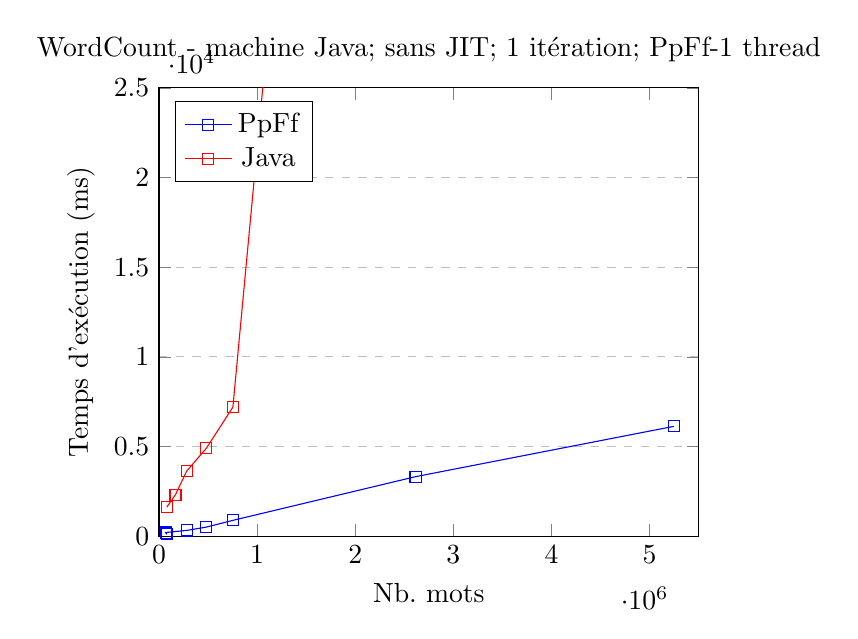
\begin{tikzpicture}
\begin{axis}[
    title={WordCount - machine Java; sans JIT; 1 itération; PpFf-1 thread\bigskip},
    xlabel={Nb.~mots},
    ylabel={Temps d'ex\'ecution (ms)},
    xmin=0, xmax=5500000,
    ymin=0, ymax=25000,
    ytick={0,5000,10000,15000,20000,25000},
    %xtick={0,500000,1000000,1500000,3000000,4500000,5000000,5500000},
    xtick={0,1000000,2000000,3000000,4000000,5000000,6000000},
    legend pos=north west,
    ymajorgrids=true,
    grid style=dashed,
]
 
\addplot[
    color=blue,
    mark=square,
    ]
    coordinates {
    (78792,106)(67941,205)(281307,322)(482636,508)(752856,883)(2614743,3320)(5247678,6126)
    };
\addplot[
    color=red,
    mark=square,
    ]
    coordinates {
    (78792,1615)(167941,2319)(281307,3625)(482636,4906)(752856,7195)(2614743,116039)(5247678,226917)
    };
\legend{PpFf,Java}    
\end{axis}
\end{tikzpicture}



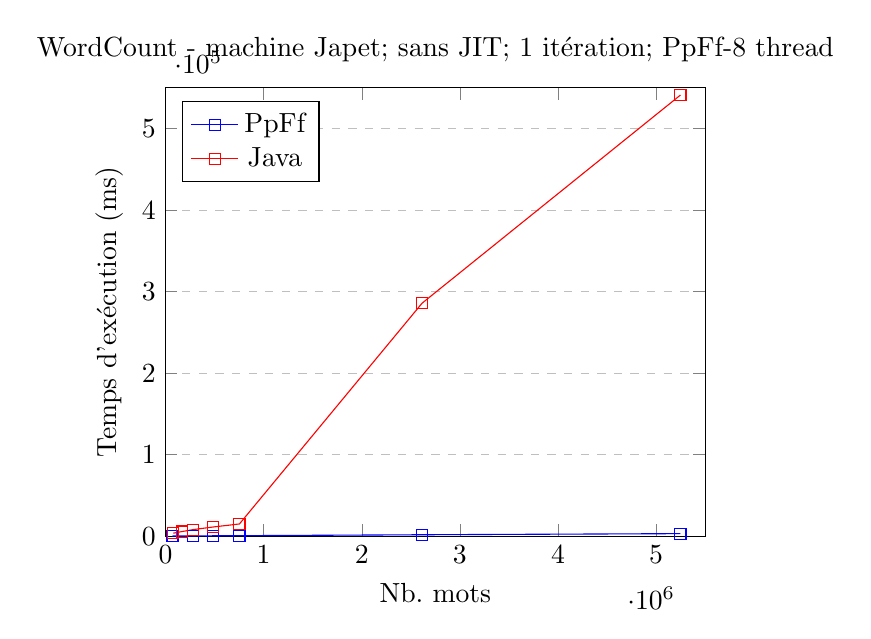
\begin{tikzpicture}
\begin{axis}[
    title={WordCount - machine Japet; sans JIT; 1 itération; PpFf-8 thread\newline},
    xlabel={Nb.~mots},
    ylabel={Temps d'ex\'ecution (ms)},
    xmin=0, xmax=5500000,
    ymin=0, ymax=550000,
    %ytick={0,100000,150000,200000,250000,300000,350000,400000,450000,500000,550000},
    ytick={0,100000,200000,300000,400000,500000,600000},
    xtick={0,1000000,2000000,3000000,4000000,5000000,6000000},
    legend pos=north west,
    ymajorgrids=true,
    grid style=dashed,
]
 
\addplot[
    color=blue,
    mark=square,
    ]
    coordinates {
    (78792,67)(67941,162)(281307,268)(482636,480)(752856,637)(2614743,1765)(5247678,3135)
    };
\addplot[
    color=red,
    mark=square,
    ]
    coordinates {
    (78792,3685)(167941,5685)(281307,8083)(482636,11258)(752856,14991)(2614743,285866)(5247678,541184)
    };
\legend{PpFf,Java}    
\end{axis}
\end{tikzpicture}






\begin{figure}[H]
\centering
	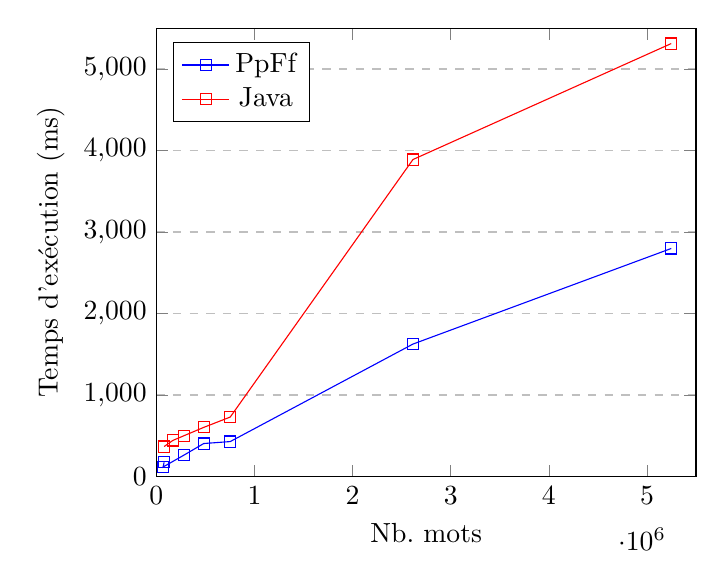
\begin{tikzpicture}
	\begin{axis}[
	    xlabel={Nb.~mots},
    	ylabel={Temps d'ex\'ecution (ms)},
	    xmin=0, xmax=5500000,
    	ymin=0, ymax=5500,
	    %ytick={0,500,1000,1500,2000,2500,3000,3500,4000,4500,5000,5500},
    	ytick={0,1000,2000,3000,4000,5000,6000},
	    xtick={0,1000000,2000000,3000000,4000000,5000000,6000000},
    	legend pos=north west,
	    ymajorgrids=true,
    	grid style=dashed,
	]
 
	\addplot[
    	color=blue,
   	 	mark=square,
    ]
    	coordinates {
    	(78792,174)(67941,117)(281307,263)(482636,405)(752856,429)(2614743,1625)(5247678,2798)
    	};
	\addplot[
    	color=red,
    	mark=square,
    ]
    	coordinates {
    	(78792,368)(167941,443)(281307,501)(482636,603)(752856,730)(2614743,3889)(5247678,5312)
    	};
	\legend{PpFf,Java}    
	\end{axis}
	\end{tikzpicture}
    \caption{Les temps d'ex\'ecution pour \TT{WordCount} sur la machine Japet.}
    \label{JapetExecutionWordCount.fig}	
\end{figure}


\begin{figure}[H]
\centering
     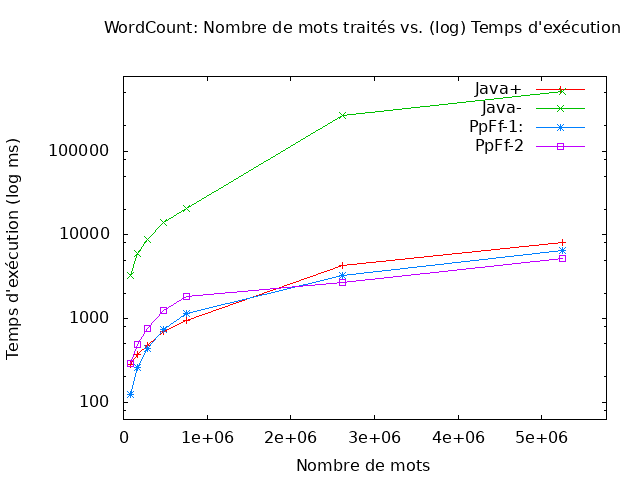
\includegraphics[width=1.0\textwidth]{Figures/GrapheTempsWordCount.png}
      \caption{Les temps d'ex\'ecution pour \TT{WordCount} sur la machine \M1.}
       \label{GrapheTempsWordCount.fig}
\end{figure}


\GT{Ci-bas: ultimement, il faudra pr\'esenter dans le texte dans le
m\^eme ordre que les num\'eros, donc 4.1 avant 4.2!}

Dans cette section, nous présentons une \'evaluation exp\'erimentale approfondie pour les op\'erations d\'ecrites dans la section pr\'ec\'edente. Nous \'evaluons l'application \TT{WordCount} \`a l'aide des m\'etriques suivantes: le nombre de mots comme valeur d'entr\'ee et le temps en millisecondes comme valeur de sortie. Afin de conna\^itre l'impact de la quantit\'e de donn\'ees \`a traiter, les exp\'eriences ont \'et\'e men\'ees en utilisant plusieurs ensembles de donn\'ees. Chaque ensemble de donn\'ees est repr\'esent\'e par un nombre de mots contenus dans un fichier sur disque. Les nombres de mots de chaque fichier varient de 78~792 \`a 5~247~678. Pour toutes les exp\'eriences, le facteur de r\'ep\'etitions a \'et\'e \'etabli \`a 20.  Les r\'esultats sont pr\'esent\'es dans les figures~\ref{GrapheTempsWordCount.fig} et~\ref{JapetExecutionWordCount.fig} respectivement. La figure~\ref{GrapheTempsWordCount.fig} montre les résultats obtenus sur la machine \M1\ et la figure~\ref{JapetExecutionWordCount.fig} montre les r\'esultats obtenus sur la machine M2 (p.~\pageref{machines.sect}).

Deux s\'eries d'exp\'eriences ont \'et\'e men\'ees dans le cas de \TT{Java}. L'une avec \emph{JIT} et l'autre sans (p.~\pageref{jitDescription.sect}). On constate que le temps d'ex\'ecution de \TT{WordCount} sans \emph{JIT} est nettement sup\'erieure \`a celui avec \emph{JIT}.

Dans le cas de \TT{PpFf}, les exp\'eriences ont \'et\'e men\'ees en variant les nombres de \emph{threads}. Le temps d'ex\'ecution de \TT{PpFf} avec un \emph{thread} par rapport \`a celui avec deux \emph{threads} est meilleur lorsque la charge du travail est petite. La m\^eme situation peut \^etre constat\'ee lorsqu'on compare le temps d'ex\'ecution de \TT{PpFf} avec celui de \TT{Java}. Pour un petit nombre de mots \`a traiter, le temps d'ex\'ecution de \TT{Java} est meilleur. Cela peut s'expliquer par le mode de construction diff\'erent du pipeline entre les deux programmes. En comparaison avec \TT{Java}, \TT{PpFf} ex\'ecute chaque op\'eration d'un \TT{pipeline} sur un \emph{thread} diff\'erent. Par exemple, les cinq op\'erations de \TT{WordCount} --- \TT{source}, \TT{flatMap}, \TT{map}, \TT{find} et \TT{reduceByKey} --- s'ex\'ecutent sur cinq \emph{threads} diff\'erents. Les co\^uts suppl\'ementaires introduits par ces \emph{threads} sont refl\'et\'es dans un moins bon temps d'ex\'ecution pour une petite charge du travail. Par contre, lorsque la charge du traitement est grande, \TT{PpFf} obtient un meilleur temps d'ex\'ecution que \TT{Java}.



\section{Stock Market}
\label{stockprice.sect}

\gt{En anglais <<stock>> est, en fran\c{c}ais, une <<action (boursi\`ere)>>.}

Dans le monde informatique actuel, les institutions financi\`eres produisent d'\'enormes quantit\'es d'informations, par ex., les informations sur les march\'es boursiers. Un probl\`eme important qu'elles rencontrent consiste \`a trouver des moyens efficaces pour r\'esumer et visualiser les donn\'ees afin de produire des informations utiles sur le comportement du march\'e, notamment pour prendre des d\'ecisions d'investissement. Cette section pr\'esente une application qui calcule le prix maximum pour diverses actions d'un marché boursier. Les codes sources des applications \TT{StockPrice} en \TT{PpFf} et~\TT{Java} sont pr\'esent\'es dans les annexes~\ref{sourceCodeStockPricePpFf.ann} et~\ref{sourceCodeStockPriceJava.ann} respectivement. 

\subsection{Description de l'application}

L'application \TT{Stock Market} calcule le prix d'une action en utilisant le modèle \emph{Black-Scholes}~\citep{macbeth1979empirical}. Ce mod\`ele d'\'evaluation est utilis\'e pour d\'eterminer le prix juste ou la valeur th\'eorique d'une option d'achat ou de vente, et ce en fonction de six variables telles que la valeur de l'action sous-jacente, le prix d'exercice, le taux d'int\'er\^et sans risque, la volatilit\'e du prix de l'action, la dur\'ee et le type d'option. 

L'application \TT{Stock Market} est compos\'ee de cinq op\'erations principales~: 

\begin{lstlisting}[
label={exampleInfoActionFromFile},
language=c++,
caption={Un exemple illustrant l'information sur des actions contenues dans le fichier.},
frame=single,
float]
SNY 100.00 90.00 0.1000 0.00 0.10 1.00 C 0.00 18.6308591206674982
JCI 100.00 100.00 0.1000 0.00 0.10 0.50 C 0.00 5.8502736042849798
DSX 100.00 100.00 0.1000 0.00 0.10 1.00 C 0.00 10.3081472436668
LILA 100.00 110.00 0.1000 0.00 0.10 0.10 C 0.00 0.003523074865
NVS 100.00 110.00 0.1000 0.00 0.10 0.50 C 0.00 1.1407228438274099
FLML 100.00 110.00 0.1000 0.00 0.10 1.00 C 0.00 4.216747020308
TEF 100.00 90.00 0.1000 0.00 0.25 0.10 C 0.00 11.1352446183467002
DXB 100.00 90.00 0.1000 0.00 0.25 0.50 C 0.00 16.0926388440922991
HSEA 100.00 90.00 0.1000 0.00 0.25 1.00 C 0.00 21.16345465848
LENS 100.00 100.00 0.1000 0.00 0.25 0.10 C 0.00 3.65996266031
\end{lstlisting}

\begin{itemize}

\item Une op\'eration qui d\'efinit la source du flux de donn\'ees. Ici, la source est constitu\'ee par les lignes contenues dans un fichier. Le listing~\ref{exampleInfoActionFromFile} montre un exemple avec quelques enregistrements tir\'es de notre fichier de test. 

Un enregistrement est identifi\'e par les informations suivantes : le nom de l'action, la valeur actuelle de l'action sous-jacente, le prix d'exercice, le taux d'int\'er\^et sans risque, le taux de dividende, la volatilit\'e du prix de l'action, le temps qu'il reste \`a l'option avant son \'ech\'eance (exprim\'e en ann\'ees), le type d'option (\TT{C=CALL}~: prix pour une option d'achat et \TT{P=PUT}~: prix pour une option de vente), la valeur de dividende et la valeur de r\'ef\'erence \TT{DerivaGem}. 
Les valeurs \TT{DerivaGem}, la valeur et le taux de dividende ne sont pas utilis\'es dans \TT{Stock Market} pour calculer le prix d'une action.

\item Une op\'eration qui r\'epartit les \'el\'ements du flux entre divers \emph{threads}.
Toutes les \'etapes qui suivent cette op\'eration seront donc ex\'ecut\'ees en parall\`ele.

\item Une op\'eration  \TT{map}, qui permet d'extraire le nom et les options de chaque action.

\gt{En fait, que contient un enregistrement: les infos sur une action
sp\'ecifique? Ou une transaction boursi\`ere? \`A clarifier!}

\ic{Bonne question. J'imagine qu'il s'agit d'actions enregistr\'ees \`a la suite de transaction boursi\`ere. J'ai regard\'e la description de Pico. Il n'y a pas beaucoup de d\'etails. https://github.com/alpha\-unito/pico/tree/master/examples/stock-market. (The stock\_pricing.cpp code is an example of batch pipeline (like word\-count), meaning file\-based I\/O. It takes in input a series of stock records and computes the maximum price for each stock name.) }

\item  Une op\'eration qui calcule le prix de chaque action. L'algorithme utilis\'e est celui de \emph{Black \& Scholes}~\citep{macbeth1979empirical}. 

\item Une derni\`ere op\'eration qui extrait le prix maximum pour chaque action.


\end{itemize}

\subsection{Mesures obtenues et analyse des r\'esultats}


\pgfplotstableread[row sep=\\,col sep=&]{
    interval & PpFf & Java \\
    M1+  & 302 & 574 \\
    M1-   & 504 & 2696 \\
    M2+   & 357 & 402 \\
    M2-   & 350 & 5810 \\
    }\mydata

\begin{figure}[H]
\centering
	\begin{tikzpicture}
    	\begin{axis}[
            ybar,
            bar width=.5cm,
            width=.7\textwidth,
            height=.5\textwidth,
            legend style={at={(0.5,1)},
                anchor=north,legend columns=-1},
            symbolic x coords={M1+, M1-, M2+, M2-},
            xtick=data,
            nodes near coords,
            nodes near coords align={vertical},
            ymin=0,ymax=6000,
            ylabel={Temps d'ex\'ecution (ms)},
        ]
        \addplot table[x=interval,y=PpFf]{\mydata};
        \addplot table[x=interval,y=Java]{\mydata};
        \legend{PpFf, Java}
    	\end{axis}
	\end{tikzpicture}
    \caption{Les temps d'ex\'ecution pour l'application \TT{Stock Market}.}
    \label{executionTimesStockPrice.fig}
\end{figure}

\GT{Quand tu parles des exp\'eriences que tu as faites --- donc dans
le pass\'e --- tu dois \'ecrire au pass\'e.  Par contre, tu peux
\'ecrire au pr\'esent pour l'analyse des r\'esultats.}

La deuxi\`eme s\'erie d'exp\'eriences pour analyser les performances de \PpFf{} a \'et\'e men\'ee pour l'application permettant de calculer des statistiques sur les prix d'indices boursiers. Les r\'esultats sont pr\'esent\'es dans la figure~\ref{executionTimesStockPrice.fig}. Les expériences ont \'et\'e menées sur les deux machines \M1, \M2\ (Sect.~\ref{machines.sect}). Dans les deux cas, \TT{PpFf} obtient de meilleurs temps d'ex\'ecution en comparaison avec \TT{Java}.


\section{Surco\^uts introduits par \TT{PpFf}}
\label{coutsPpFf.sect}

\GT{On parle ici de <<surco\^uts>> --- \emph{overhead}.}

D\'ecrit dans le chapitre~\ref{implementation.chap}, \TT{PpFf} est impl\'ement\'e au-dessus de la biblioth\`eque \TT{FastFlow}. Cette section pr\'esente les surco\^uts introduits par \TT{PpFf} par rapport \`a \TT{FastFlow}. 


\subsection{Description de l'application}

Pour cette exp\'erience, nous avons cr\'e\'e un \emph{micro benchmark} consistant en un {pipeline} avec un seul op\'erateur. L'op\'erateur choisi pour cette exp\'erience est un \TT{map} qui fait un simple calcul it\'eratif, qui incr\'emente  \TT{nb} fois une variable \TT{*res}, o\`u \TT{nb}~=~$10^{\TT{granularity}}$~:
{
\begin{lstlisting}[language=c++]
  int nb = pow(10, granularity);
  for (int i = 1; i <= nb; i++) {
    *res += 1;   
  }
\end{lstlisting}
} 

Ici, \TT{granularity} est un param\`etre sp\'ecifi\'e en argument lors du lancement de l'application. Les codes sources de cette application pour~\TT{PpFf} et~\TT{FastFlow} sont pr\'esent\'es en annexe (Annexes~\ref{sourceCodeMicrobenchmarkPpFf.ann} et~\ref{sourceCodeMicrobenchmarkFastFlow.ann} respectivement). Le m\^eme calcul se r\'ep\`ete pour chaque \'el\'ement dans le \TT{pipeline}. La source du \TT{pipeline} est constitu\'ee d'une suite d'\'el\'ements. Pour cette exp\'erience, la suite est compos\'ee des entiers allant de 1 \`a 100~000.  


\subsection{Mesures obtenues et analyse des r\'esultats}

Afin d'identifer les surco\^uts introduits par \PpFf{} par rapport \`a \TT{FastFlow}, deux s\'eries d'exp\'eriences ont \'et\'e men\'ees~: une avec \TT{granularity = 4}, l'autre avec \TT{granularity~=~5}. Pour la suite d'entiers allant de 1 \`a 100~000, les exp\'eriences ont \'et\'e r\'ealis\'ees avec un nombre variable de \emph{threads} sur deux machines diff\'erentes : \M1\ et M2\ (Sect.~\ref{machines.sect}).  

\begin{figure}[H]
\centering
	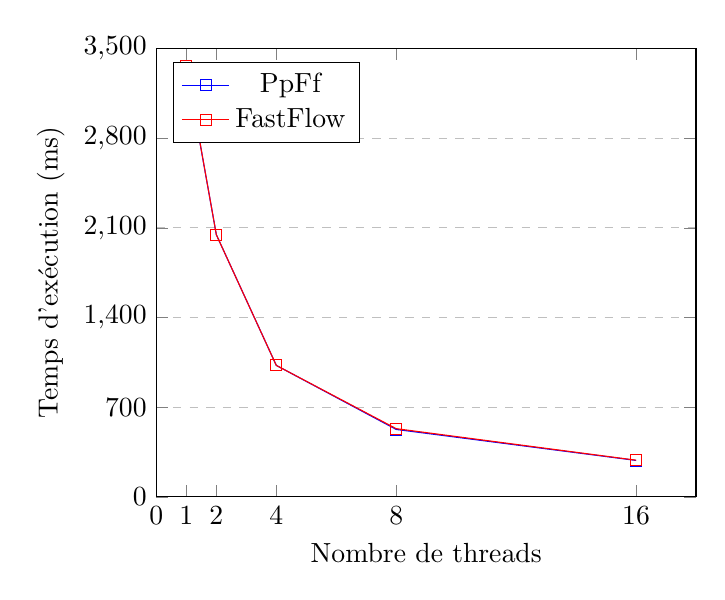
\begin{tikzpicture}
	\begin{axis}[
	    xlabel={Nombre de threads},
    	ylabel={Temps d'ex\'ecution (ms)},
	    xmin=0, xmax=18,
    	ymin=0, ymax=3500,
	    ytick={0,700,1400,2100,2800,3500},
	    xtick={0,1,2,4,8,16},
    	legend pos=north west,
	    ymajorgrids=true,
    	grid style=dashed,
	]
 
	\addplot[
    	color=blue,
   	 	mark=square,
    ]
    	coordinates {
    	(1,3360)(2,2046)(4,1026)(8,526)(16,284)
    	};
	\addplot[
    	color=red,
    	mark=square,
    ]
    	coordinates {
    	(1,3365)(2,2046)(4,1026)(8,532)(16,286)
    	};
	\legend{PpFf,FastFlow}    
	\end{axis}
	\end{tikzpicture}
    \caption{Les temps d'ex\'ecution pour \TT{MicroBenchmarkMaps} Map 1 et granularit\'e 4 sur la machine Japet.}
    \label{JapetExecutionMicroBenchmarkGr4.fig}	
\end{figure}





\begin{figure}[H]
\centering
	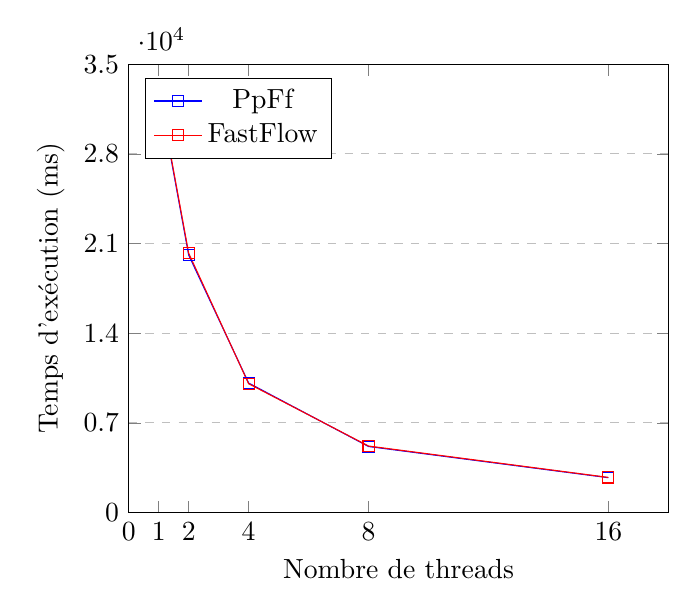
\begin{tikzpicture}
	\begin{axis}[
	    xlabel={Nombre de threads},
    	ylabel={Temps d'ex\'ecution (ms)},
	    xmin=0, xmax=18,
    	ymin=0, ymax=35000,
	    ytick={0,7000,14000,21000,28000,35000},
	    xtick={0,1,2,4,8,16},
    	legend pos=north west,
	    ymajorgrids=true,
    	grid style=dashed,
	]
 
	\addplot[
    	color=blue,
   	 	mark=square,
    ]
    	coordinates {
    	(1,32905)(2,20100)(4,10107)(8,5154)(16,2718)
    	};
	\addplot[
    	color=red,
    	mark=square,
    ]
    	coordinates {
    	(1,33028)(2,20246)(4,10055)(8,5189)(16,2740)
    	};
	\legend{PpFf,FastFlow}    
	\end{axis}
	\end{tikzpicture}
    \caption{Les temps d'ex\'ecution pour \TT{MicroBenchmarkMaps} Map 1 et granularit\'e 5 sur la machine Japet.}
    \label{JapetExecutionMicroBenchmarkGr5.fig}	
\end{figure}






\begin{figure}[H]
\centering
	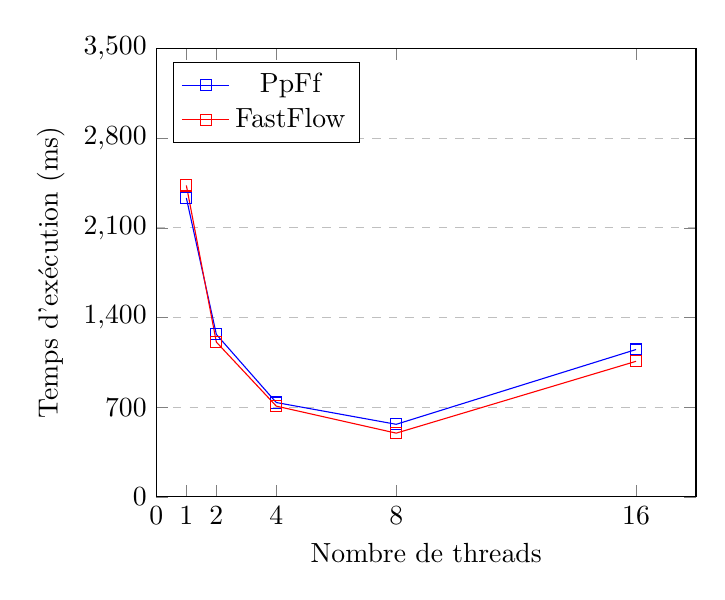
\begin{tikzpicture}
	\begin{axis}[
	    xlabel={Nombre de threads},
    	ylabel={Temps d'ex\'ecution (ms)},
	    xmin=0, xmax=18,
    	ymin=0, ymax=3500,
	    ytick={0,700,1400,2100,2800,3500},
	    xtick={0,1,2,4,8,16},
    	legend pos=north west,
	    ymajorgrids=true,
    	grid style=dashed,
	]
 
	\addplot[
    	color=blue,
   	 	mark=square,
    ]
    	coordinates {
    	(1,2333)(2,1268)(4,736)(8,566)(16,1150)
    	};
	\addplot[
    	color=red,
    	mark=square,
    ]
    	coordinates {
    	(1,2431)(2,1208)(4,708)(8,497)(16,1058)
    	};
	\legend{PpFf,FastFlow}    
	\end{axis}
	\end{tikzpicture}
    \caption{Les temps d'ex\'ecution pour \TT{MicroBenchmarkMaps} Map 1 et granularit\'e 4 sur la machine Java.}
    \label{JavatExecutionMicroBenchmarkGr4.fig}	
\end{figure}





\begin{figure}[H]
\centering
	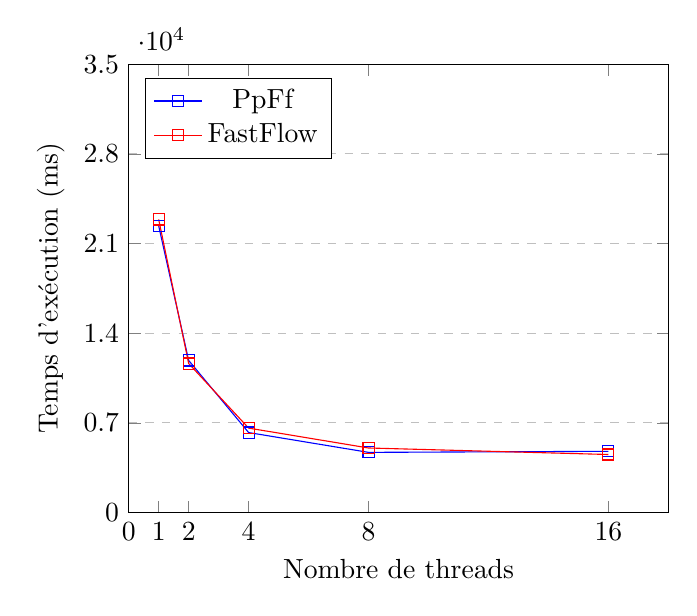
\begin{tikzpicture}
	\begin{axis}[
	    xlabel={Nombre de threads},
    	ylabel={Temps d'ex\'ecution (ms)},
	    xmin=0, xmax=18,
    	ymin=0, ymax=35000,
	    ytick={0,7000,14000,21000,28000,35000},
	    xtick={0,1,2,4,8,16},
    	legend pos=north west,
	    ymajorgrids=true,
    	grid style=dashed,
	]
 
	\addplot[
    	color=blue,
   	 	mark=square,
    ]
    	coordinates {
    	(1,22377)(2,11872)(4,6242)(8,4695)(16,4778)
    	};
	\addplot[
    	color=red,
    	mark=square,
    ]
    	coordinates {
    	(1,22879)(2,11630)(4,6590)(8,5037)(16,4529)
    	};
	\legend{PpFf,FastFlow}    
	\end{axis}
	\end{tikzpicture}
    \caption{Les temps d'ex\'ecution pour \TT{MicroBenchmarkMaps} Map 1 et granularit\'e 5 sur la machine Java.}
    \label{JavaExecutionMicroBenchmarkGr5.fig}	
\end{figure}


\GT{Il serait pr\'ef\'erable de pr\'esenter dans l'ordre, tant les figures que la description dans le texte --- \M1\ avant M2.}

Les figures~\ref{JapetExecutionMicroBenchmarkGr4.fig} et~\ref{JapetExecutionMicroBenchmarkGr5.fig} montrent les r\'esultats des exp\'eriences sur la machine \M2\ alors que les figures~\ref{JavatExecutionMicroBenchmarkGr4.fig} et~\ref{JavaExecutionMicroBenchmarkGr5.fig} montrent les r\'esultats des exp\'eriences sur la machine \M1. On constate un faible surco\^ut introduit par \PpFf\ sur la machine \M1. \TT{FastFlow} obtient un meilleur temps d'ex\'ecution pour un nombre de \emph{threads} plus grand que 8. La plus grande diff\'erence obtenue entre les temps d'ex\'ecutions de \TT{PpFf} et \TT{FastFlow} est de 100 ms. En prenant en consid\'eration le volume de traitement des deux applications, les surco\^uts introduits par \TT{PpFf} par rapport \`a \TT{FastFlow} sont donc faibles.




